{\textbf{1. 对称矩阵}}

{将对称矩阵A压缩存储到SA{[}n(n+1)/2{]}中,aij的下标i、j与在SA中的对应元素的下标k的关系如下:}

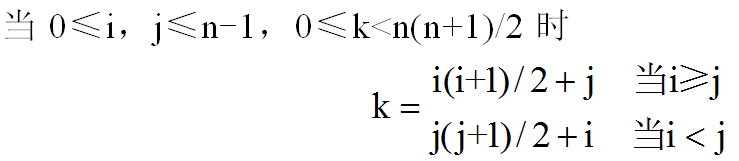
\includegraphics[width=2.50000in,height=0.54167in]{png-jpeg-pics/923EFD19FF65BD5EDFECF4ADEC3A717D.png}

{\textbf{2. 三角矩阵}}

{将上三角矩阵A压缩存储到SA{[}n(n+1)/2{]}中,aij的下标i、j与在SA中的对应元素的下标k的关系如下:}

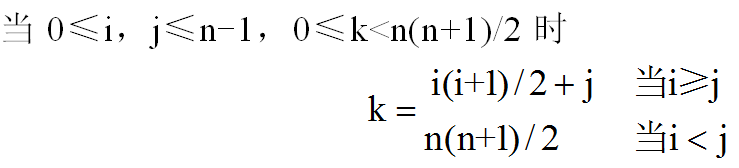
\includegraphics[width=2.39583in,height=0.54167in]{png-jpeg-pics/E7283989C6C7D818334F39947B9EEB2A.png}

{下三角{矩阵A压缩存储到SA{[}n(n+1)/2{]}中},读者可自行给出。}

{\textbf{3. 对角矩阵}}

{{所有的非零元素集中在以主对角线为中心的带状区域中},即\textbf{除了主对角线和主对角线相邻两侧的若干条对角线上的元素之外,其余元素皆为零的矩阵称为对角矩阵}。}

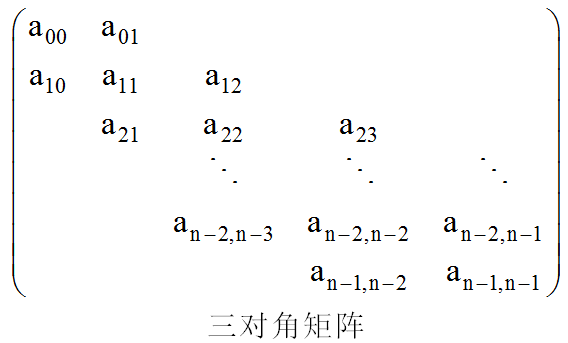
\includegraphics[width=2.29167in,height=1.38542in]{png-jpeg-pics/484F3A07CB60CCCB7EB5FBD84C919F57.png}
